\documentclass[11pt,a4paper]{article}

% ---------- Packages ----------
\usepackage[margin=0.82in,headheight=22pt,headsep=18pt,footskip=24pt]{geometry}
\usepackage[T1]{fontenc}
\usepackage{lmodern}
\usepackage{microtype}
\usepackage{amsmath,amssymb,mathtools}
\usepackage{graphicx}
\usepackage{booktabs,tabularx,array}
\usepackage{float}
\usepackage{subcaption}
\usepackage{xcolor}
\usepackage{listings}
\usepackage{fancyhdr}
\usepackage[hidelinks]{hyperref}

% ---------- Colours and page style ----------
\definecolor{navy}{RGB}{31,57,100}
\definecolor{pale}{RGB}{235,241,250}
\definecolor{codegray}{RGB}{110,110,110}
\pagestyle{fancy}
\fancyhf{}
\fancyhead[L]{\small\color{navy}Maximum Likelihood Estimation}
\fancyhead[R]{\small Abhay Sachan}
\renewcommand{\headrulewidth}{0.45pt}
\fancyfoot[C]{\thepage}
\setlength{\parindent}{1.2em}
\setlength{\parskip}{3pt}

\lstdefinestyle{pythonstyle}{
  language=Python,
  basicstyle=\ttfamily\small,
  keywordstyle=\color{navy}\bfseries,
  commentstyle=\color{codegray}\itshape,
  stringstyle=\color{teal!70!black},
  numbers=left,
  numberstyle=\tiny\color{gray},
  numbersep=7pt,
  frame=single,
  breaklines=true,
  showstringspaces=false,
  tabsize=4,
  xleftmargin=1em,
  framexleftmargin=0.5em
}

\title{Maximum Likelihood Estimation for Linear Regression}
\author{Abhay Sachan}
\date{October 2026}

\begin{document}

% ---------- Cover page ----------
\begin{titlepage}
  \thispagestyle{empty}
  \centering
  \vspace*{1.0cm}
  {\Large\bfseries UPES, Dehradun\par}
  \vspace{0.25cm}
  {\large School of Computer Science -- Artificial Intelligence Cluster\par}
  \vspace{1.5cm}
  {\Large\color{navy}APPLIED MACHINE LEARNING (CSAI2017P)\par}
  \vspace{0.7cm}
  {\huge\bfseries Maximum Likelihood Estimation\par}
  \vspace{0.3cm}
  {\LARGE Gaussian Linear Regression\par}
  \vspace{1.2cm}
  {\large Mid-Semester Assignment Report\par}
  \vspace{1.0cm}
  \renewcommand{\arraystretch}{1.5}
  \begin{tabular}{rl}
    Student: & \textbf{Abhay Sachan}\\
    Batch: & \textbf{22}\\
    Unit: & \textbf{V}\\
    Topic No.: & \textbf{16}\\
    Semester: & III (Aug--Dec 2026)\\
    Submitted to: & Kunwar Siddharth, Assistant Professor\\
    Date: & October 16, 2026\\
    Topic: & Maximum Likelihood Estimation for Regression
  \end{tabular}
  \vfill
  {\large Mathematical Derivation \quad Numerical Example \quad Python Demonstration\par}
\end{titlepage}

\pagenumbering{roman}
\begin{abstract}
Maximum Likelihood Estimation (MLE) is a statistical method for selecting model parameters that make observed data most plausible under an assumed probability distribution. This report introduces MLE through simple linear regression with independent Gaussian errors. It develops the likelihood and log-likelihood functions, derives the maximum-likelihood estimates of the regression coefficients and error variance, and explains why the coefficient estimates coincide with ordinary least squares under the Gaussian assumption. A reproducible Python demonstration generates a small synthetic dataset, fits a regression line, estimates the noise variance, and plots a profile negative log-likelihood curve. The example illustrates how likelihood turns a probabilistic model into an estimation procedure. The report also discusses computational complexity, assumptions, limitations, and practical applications. The numerical values are specific to the fixed synthetic dataset used in the demonstration; they are not claims about a real-world dataset.
\end{abstract}

\tableofcontents
\clearpage
\pagenumbering{arabic}

\section{Introduction}
Many machine-learning tasks require a model to learn unknown parameters from observed data. For example, a model may estimate the relationship between hours studied and an exam score, or between advertising expenditure and sales. The data contain variation, so the model needs a principled way to choose parameter values.

Maximum Likelihood Estimation (MLE) provides one such method. We begin by specifying a probability model for the observations. MLE then chooses the parameter values that maximize the likelihood of the observed dataset under that model \cite{casella,murphy}. For continuous observations, likelihood is a density evaluated at the observed values; it should not be interpreted as the probability of observing one exact real number.

This report studies MLE for simple linear regression when errors are independent and normally distributed with a common variance. This example is useful because it gives clear formulas, a hand-solvable derivation, and a short Python implementation. The Gaussian assumption is important: under it, the maximum-likelihood coefficient estimates equal the ordinary least-squares estimates, while the MLE of the variance divides the residual sum of squares by the number of observations \cite{bishop,murphy}.

\section{Intuition and Core Idea}
Suppose data points are scattered around an unknown straight line. A line that passes close to the observations usually leaves smaller residuals than a poor line. If we assume the residuals follow a Gaussian distribution, the model assigns higher likelihood to parameter values that keep the residuals collectively small, while also accounting for the noise variance.

Let $x_i$ be the input, $y_i$ the observed response, $\beta_0$ the intercept, $\beta_1$ the slope, and $\sigma^2$ the error variance. The model is
\[
y_i=\beta_0+\beta_1x_i+\epsilon_i,\qquad
\epsilon_i\overset{\mathrm{iid}}{\sim}\mathcal{N}(0,\sigma^2).
\]
The parameters are not known in advance. MLE finds the values of $\beta_0$, $\beta_1$, and $\sigma^2$ that maximize the joint likelihood of the observations.

\begin{figure}[H]
\centering
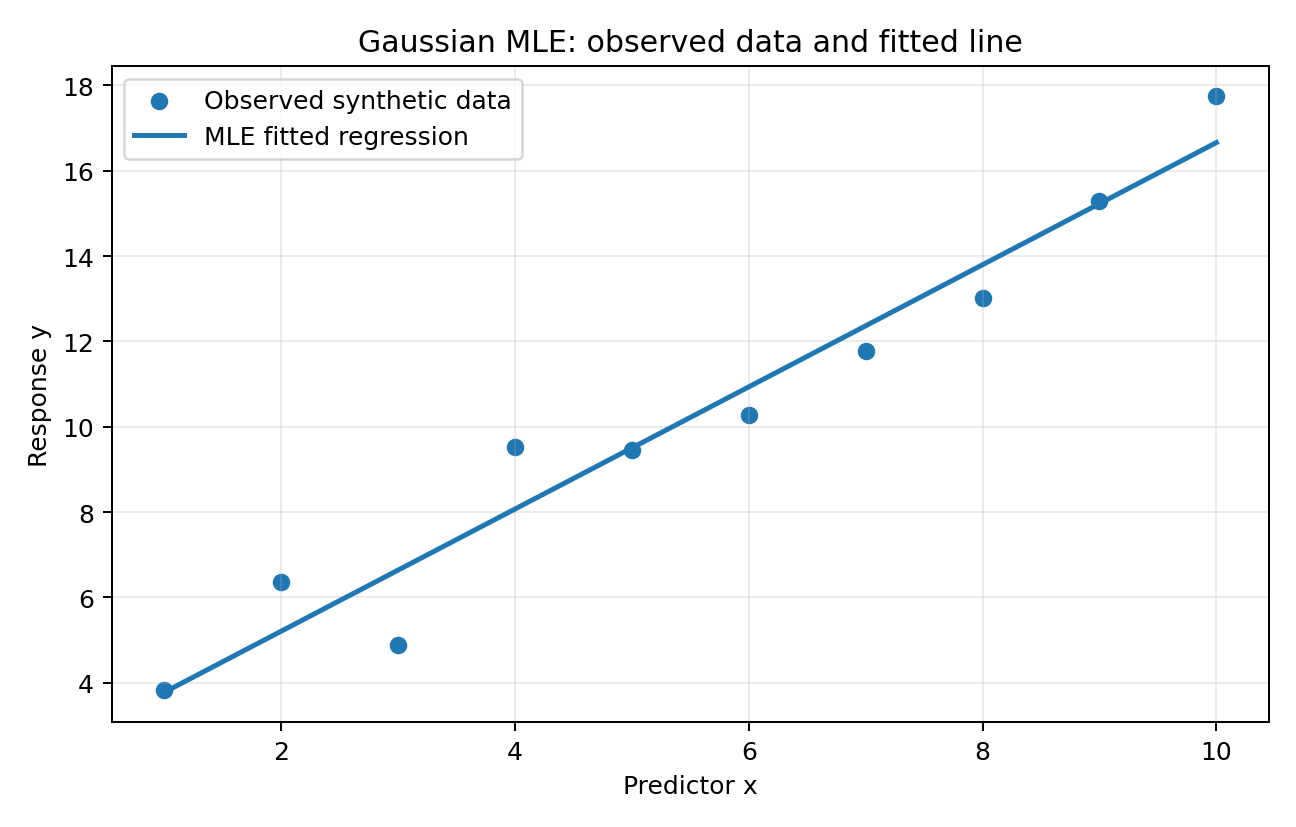
\includegraphics[width=0.78\textwidth]{figures/fit.png}
\caption{Synthetic observations and the fitted regression line produced by the Python demonstration.}
\label{fig:fit}
\end{figure}

\noindent\textbf{Key idea.} MLE chooses parameters by maximizing the likelihood of the observed data under an assumed probability model. For Gaussian linear regression, maximizing the likelihood over the coefficients is equivalent to minimizing the sum of squared residuals.

\section{Mathematical Formulation}
\subsection{Model and assumptions}
For $n$ observed pairs $(x_i,y_i)$, assume
\begin{equation}
y_i=\beta_0+\beta_1x_i+\epsilon_i,\qquad
\epsilon_i\overset{\mathrm{iid}}{\sim}\mathcal{N}(0,\sigma^2),\quad \sigma^2>0.
\label{eq:model}
\end{equation}
The observations are conditionally independent given the inputs and parameters. The model assumes a linear conditional mean, zero-mean Gaussian errors, and constant error variance. The slope is identifiable when the input values are not all identical.

\subsection{Likelihood and log-likelihood}
For each observation, the conditional density is
\begin{equation}
p(y_i\mid x_i,\beta_0,\beta_1,\sigma^2)
=\frac{1}{\sqrt{2\pi\sigma^2}}
\exp\left[-\frac{(y_i-\beta_0-\beta_1x_i)^2}{2\sigma^2}\right].
\label{eq:density}
\end{equation}
By independence, the likelihood of the complete dataset is the product of these densities:
\begin{equation}
L(\beta_0,\beta_1,\sigma^2)
=\prod_{i=1}^{n}p(y_i\mid x_i,\beta_0,\beta_1,\sigma^2).
\label{eq:likelihood}
\end{equation}
Taking the natural logarithm gives the log-likelihood
\begin{align}
\ell(\beta_0,\beta_1,\sigma^2)
&=-\frac{n}{2}\log(2\pi)-\frac{n}{2}\log(\sigma^2) \nonumber\\
&\quad-\frac{1}{2\sigma^2}\sum_{i=1}^{n}(y_i-\beta_0-\beta_1x_i)^2.
\label{eq:loglik}
\end{align}
The logarithm is strictly increasing, so maximizing the likelihood and maximizing the log-likelihood give the same parameter estimates. The log form is often easier to work with because it changes a product into a sum.

\subsection{Maximum-likelihood estimates of the coefficients}
For fixed $\sigma^2>0$, the first two terms of Equation~\eqref{eq:loglik} do not depend on $\beta_0$ or $\beta_1$. Therefore, maximizing the log-likelihood over these coefficients is equivalent to minimizing
\begin{equation}
S(\beta_0,\beta_1)=\sum_{i=1}^{n}(y_i-\beta_0-\beta_1x_i)^2.
\label{eq:rss}
\end{equation}
Differentiating with respect to the intercept and slope and setting the derivatives to zero yields the least-squares normal equations. Their solution is
\begin{equation}
\widehat{\beta}_1=
\frac{\sum_{i=1}^{n}(x_i-\bar{x})(y_i-\bar{y})}
{\sum_{i=1}^{n}(x_i-\bar{x})^2},
\qquad
\widehat{\beta}_0=\bar{y}-\widehat{\beta}_1\bar{x}.
\label{eq:coeff}
\end{equation}
Here, $\bar{x}$ and $\bar{y}$ are the sample means. Thus, under independent Gaussian errors, the MLEs of the intercept and slope equal the ordinary least-squares estimates.

\subsection{Maximum-likelihood estimate of variance}
Write $v=\sigma^2$. Differentiating Equation~\eqref{eq:loglik} with respect to $v$ and setting the derivative to zero gives
\[
-\frac{n}{2v}+\frac{\mathrm{RSS}}{2v^2}=0,
\]
where $\mathrm{RSS}=\sum_{i=1}^{n}(y_i-\widehat{y}_i)^2$. Solving for $v$ gives
\begin{equation}
\boxed{\widehat{\sigma}^{\,2}_{\mathrm{MLE}}
=\frac{1}{n}\sum_{i=1}^{n}(y_i-\widehat{y}_i)^2
=\frac{\mathrm{RSS}}{n}.}
\label{eq:variance}
\end{equation}
This MLE differs from the common unbiased variance estimator $\mathrm{RSS}/(n-2)$ for simple linear regression with an intercept. The difference arises because the two estimators optimize different criteria.

\section{Algorithm / Procedure}
The demonstration uses a small synthetic dataset so that results can be reproduced without downloading external data.

\noindent\textbf{Input:} Numeric pairs $(x_i,y_i)$ and the Gaussian-error assumption.\\
\textbf{Output:} Estimated intercept, slope, residual variance, and diagnostic plots.

\begin{enumerate}
\item Generate or load the observations and check that the inputs are numeric.
\item Construct the design matrix $X$ with a column of ones for the intercept and a column containing $x_i$.
\item Solve the least-squares problem to obtain $\widehat{\beta}_0$ and $\widehat{\beta}_1$.
\item Compute fitted values $\widehat{y}_i$, residuals $e_i=y_i-\widehat{y}_i$, and $\mathrm{RSS}=\sum_i e_i^2$.
\item Estimate the Gaussian error variance using $\widehat{\sigma}^2_{\mathrm{MLE}}=\mathrm{RSS}/n$.
\item Plot the observations with the fitted line and plot the profile negative log-likelihood over candidate slopes.
\end{enumerate}

\noindent\textbf{Pseudocode}
\begin{lstlisting}[basicstyle=\ttfamily\small,frame=single,breaklines=true]
Input: observations (x_i, y_i), i = 1,...,n
Build X = [ones, x]
Estimate beta = least_squares(X, y)
Compute residuals e = y - X beta
RSS = sum(e_i^2)
sigma2_MLE = RSS / n
Return beta, sigma2_MLE, fitted plot, likelihood plot
\end{lstlisting}

\section{Worked Example (Step by Step)}
The Python program uses a fixed random seed to generate ten synthetic observations from a line with intercept $2$, slope $1.5$, and Gaussian noise with standard deviation $0.9$. The true generating parameters are known for demonstration, but the estimator only sees the generated data. Because random noise is present, estimates are not expected to equal the generating values exactly.

For this run, the fitted estimates are approximately $\widehat{\beta}_0=2.3453$ and $\widehat{\beta}_1=1.4314$. The residual sum of squares is approximately $9.0398$. With $n=10$, the variance estimate is $\widehat{\sigma}^2_{\mathrm{MLE}}=9.0398/10\approx0.9040$, and the estimated standard deviation is approximately $0.9508$.

\begin{table}[H]
\centering
\small
\begin{tabularx}{\textwidth}{c X X X}
\toprule
Step & Input / activity & Result & What happened\\
\midrule
1 & Generate ten $(x_i,y_i)$ pairs & $n=10$ & A fixed seed makes the dataset reproducible.\\
2 & Fit the intercept and slope & $\widehat{\beta}_0\approx2.3453$, $\widehat{\beta}_1\approx1.4314$ & Least squares gives the Gaussian MLE coefficients.\\
3 & Calculate residuals and square them & $\mathrm{RSS}\approx9.0398$ & The residuals measure the deviations from the fitted line.\\
4 & Divide RSS by $n$ & $\widehat{\sigma}^2\approx0.9040$ & This is the Gaussian maximum-likelihood variance estimate.\\
5 & Take the square root & $\widehat{\sigma}\approx0.9508$ & The result is the estimated noise standard deviation.\\
\bottomrule
\end{tabularx}
\caption{Step-by-step trace of the numerical example. Values are rounded for display.}
\label{tab:worked}
\end{table}

The final estimates describe this particular synthetic sample. They do not prove that the data-generating parameters can be recovered exactly from every small sample. With more data and the model assumptions satisfied, estimates often become more stable, although finite-sample variation remains.

\section{Animation / Software Demonstration}
The software demonstration is implemented in Python using NumPy and Matplotlib. It produces a scatter plot with the fitted regression line, a profile negative log-likelihood plot, four key frames, and a separate animated GIF showing candidate lines moving toward the fitted line.

\noindent\textbf{Tool used:} Python 3, NumPy, and Matplotlib.\\
\textbf{What the viewer sees:} Synthetic observations, candidate regression lines, the final fitted line, and the negative log-likelihood as the candidate slope changes.\\
\textbf{What can be changed:} The random seed, sample size, noise level, or candidate-slope interval can be changed in the script. The report figures should be regenerated after edits.\\
\textbf{How to run:} Install the dependencies with \texttt{python -m pip install -r requirements.txt}, then run \texttt{python MLE.py} from the project root. The animated graph is saved as \texttt{MLE\_animation.gif} in the project root. Static figures are saved in the \texttt{figures/} directory.

\noindent\textbf{Core implementation excerpt}
\begin{lstlisting}[style=pythonstyle,caption={Estimating the coefficients and Gaussian variance}]
X = np.column_stack((np.ones_like(x), x))
beta_hat, _, _, _ = np.linalg.lstsq(X, y, rcond=None)
residuals = y - X @ beta_hat
rss = np.sum(residuals ** 2)
sigma2_hat = rss / len(x)
\end{lstlisting}

\begin{figure}[H]
\centering
\begin{subfigure}[t]{0.47\textwidth}
\centering
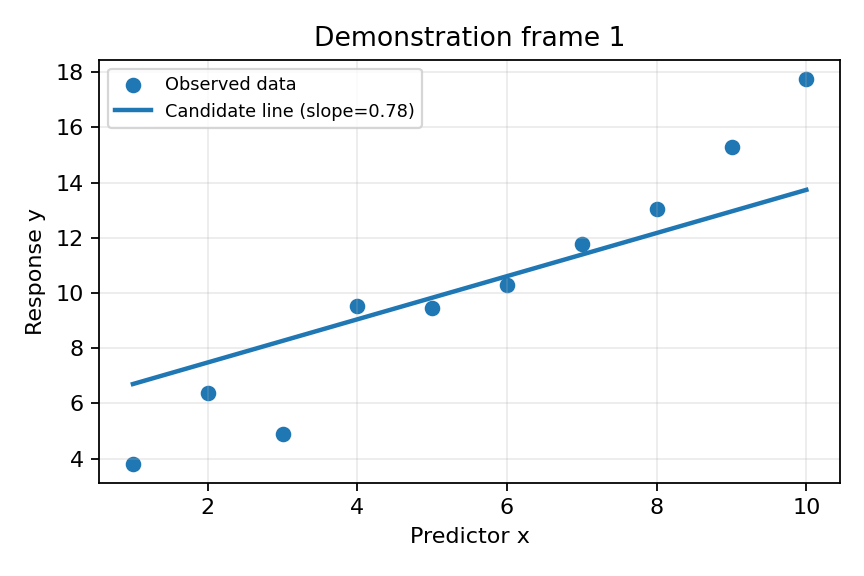
\includegraphics[width=\linewidth]{figures/frame1.png}
\caption{Candidate line before reaching the fitted slope.}
\end{subfigure}\hfill
\begin{subfigure}[t]{0.47\textwidth}
\centering
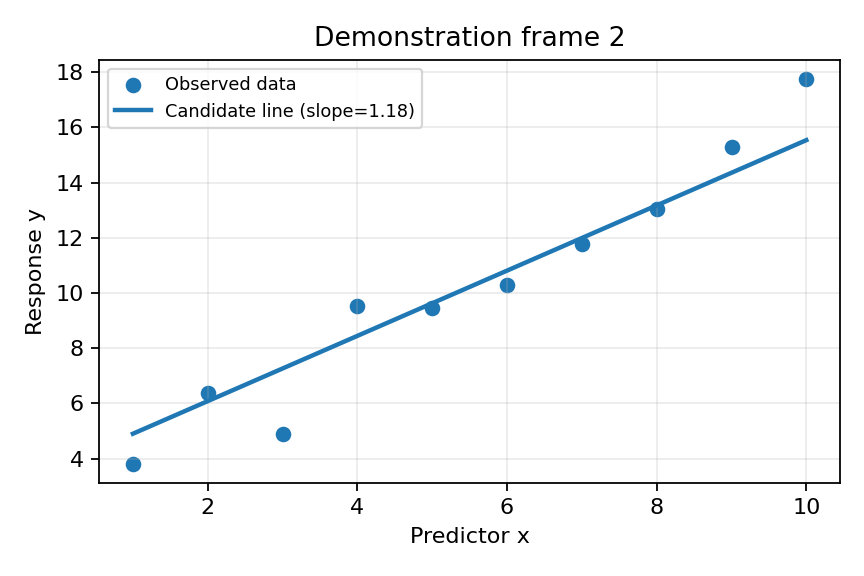
\includegraphics[width=\linewidth]{figures/frame2.png}
\caption{A candidate line closer to the fitted slope.}
\end{subfigure}

\vspace{0.4cm}
\begin{subfigure}[t]{0.47\textwidth}
\centering
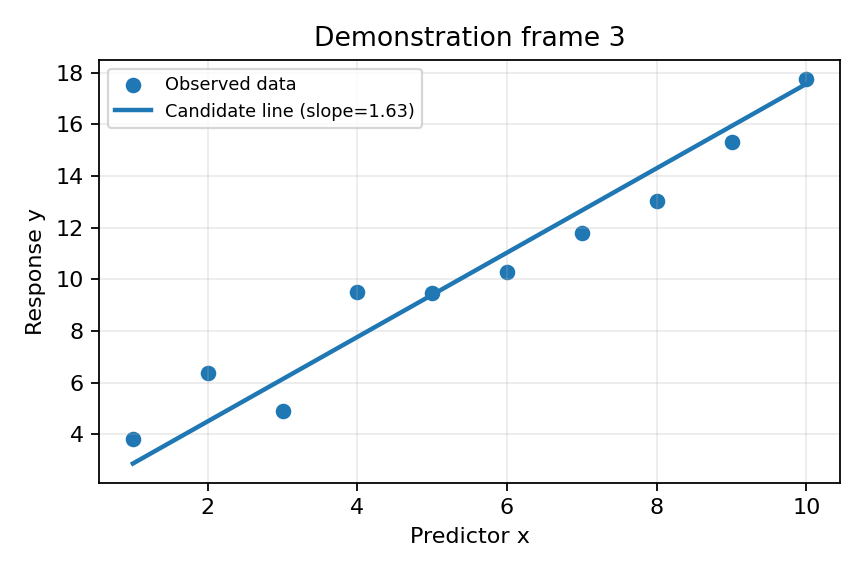
\includegraphics[width=\linewidth]{figures/frame3.png}
\caption{Another candidate line near the optimum.}
\end{subfigure}\hfill
\begin{subfigure}[t]{0.47\textwidth}
\centering
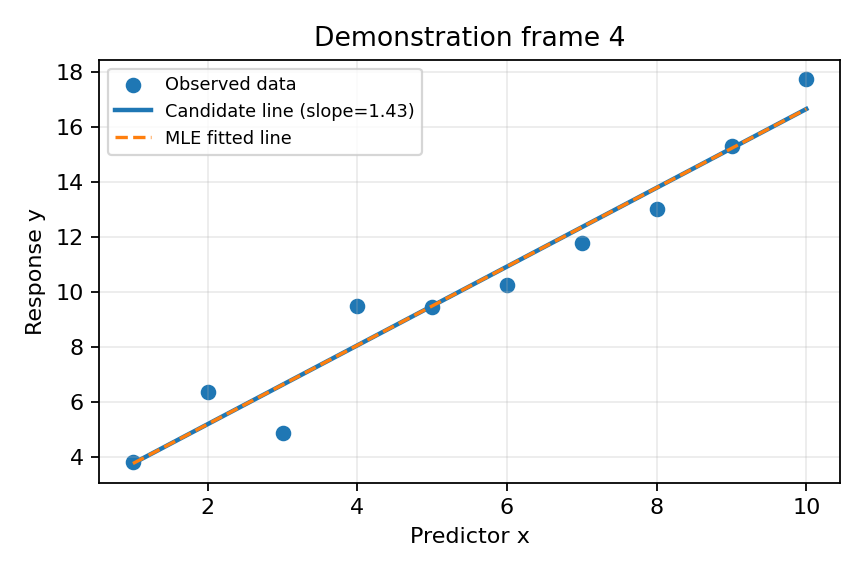
\includegraphics[width=\linewidth]{figures/frame4.png}
\caption{The maximum-likelihood fitted line.}
\end{subfigure}
\caption{Four key frames generated by the Python demonstration. These are static frames, not a continuous animation.}
\label{fig:frames}
\end{figure}

The separate file \texttt{MLE\_animation.gif} shows a continuous animation of the candidate line changing across frames; standard PDF viewers may display only the static key frames included here. Figure~\ref{fig:likelihood} complements the frames by showing the profile negative log-likelihood. The minimum marks the preferred slope after re-estimating the intercept and variance for each candidate slope.

\begin{figure}[H]
\centering
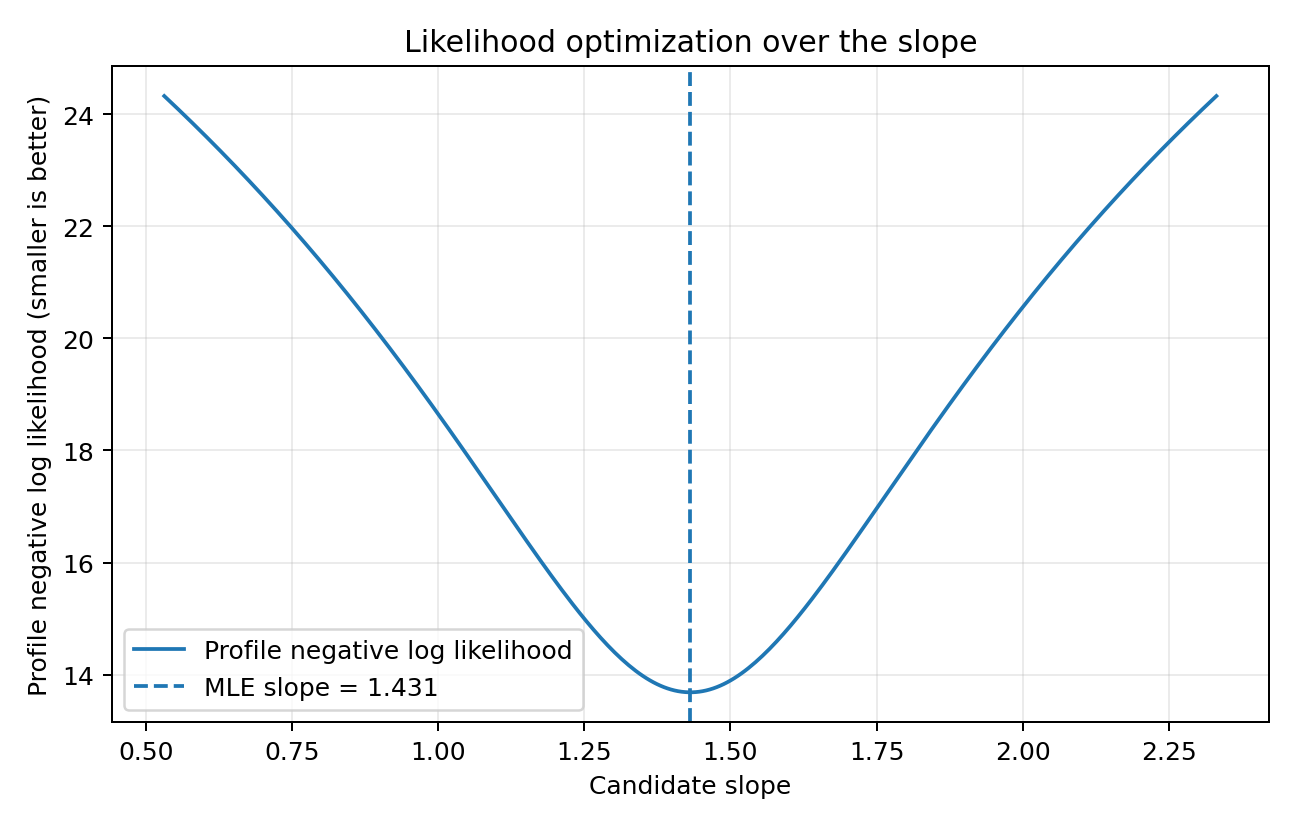
\includegraphics[width=0.78\textwidth]{figures/likelihood.png}
\caption{Profile negative log-likelihood over candidate slopes. A lower value indicates a higher likelihood for the fixed observed dataset.}
\label{fig:likelihood}
\end{figure}

\section{Analysis}
\subsection*{Time complexity}
For simple linear regression with a fixed number of parameters, accumulating the sums needed for the estimates takes $O(n)$ time. The NumPy least-squares solver also scales linearly in $n$ when the number of columns is fixed at two. The profile-likelihood plot evaluates $k$ candidate slopes, with each evaluation processing $n$ observations, so that portion takes $O(kn)$. Here, $k$ is fixed at 300, making the demonstration linear in $n$ for this implementation.

\subsection*{Space complexity}
The script stores the input arrays, design matrix, predictions, and residuals, each with $O(n)$ entries. Its overall memory use is therefore $O(n)$ for the data representation. The mathematical estimator can be computed with streaming summaries in constant auxiliary space for simple regression, but this particular demonstration retains arrays for fitting and plotting.

\subsection*{Why the method works}
The Gaussian log-likelihood in Equation~\eqref{eq:loglik} is maximized over the coefficients when the residual sum of squares is minimized. The least-squares solution therefore gives the coefficient MLEs. After substituting the fitted coefficients, differentiating the log-likelihood with respect to the positive variance yields RSS divided by $n$. These conclusions rely on the specified Gaussian model; a different noise distribution can produce a different likelihood and different estimates.

\begin{table}[H]
\centering
\small
\begin{tabularx}{\textwidth}{>{\bfseries}p{2.4cm} X X}
\toprule
Criterion & MLE for Gaussian regression & Ordinary least squares (OLS)\\
\midrule
Main goal & Maximize a specified probability model's likelihood & Minimize squared residuals\\
Coefficient estimates & Equal the OLS coefficients under Gaussian errors & Directly provide the least-squares coefficients\\
Variance estimate & $\mathrm{RSS}/n$ for Gaussian MLE & OLS alone does not require a variance estimate\\
Strength & Gives a probabilistic framework for estimation and model comparison & Simple, widely available, and easy to interpret\\
Limitation & Depends on the probability-model assumptions & Squared-error fitting can be sensitive to outliers\\
\bottomrule
\end{tabularx}
\caption{Comparison of Gaussian MLE and ordinary least squares. Their coefficient estimates coincide under the stated Gaussian model.}
\label{tab:comparison}
\end{table}

\section{Applications}
\begin{enumerate}
\item \textbf{Predictive regression:} MLE estimates regression parameters in models for sales, prices, demand, or other numerical outcomes when an appropriate noise distribution is specified.
\item \textbf{Scientific measurement:} When measurement errors are approximately Gaussian, MLE can estimate the underlying trend and the measurement-noise variance from repeated observations.
\item \textbf{Model comparison and uncertainty:} Likelihood values can support comparisons between probabilistic models and can be extended to confidence intervals, standard errors, and other uncertainty analyses when the relevant assumptions and methods are appropriate.
\end{enumerate}

\section{Conclusion}
Maximum Likelihood Estimation offers a general way to estimate parameters by selecting values that make the observed data most plausible under a probability model. In simple linear regression with independent Gaussian errors, maximizing the likelihood produces the ordinary least-squares coefficient estimates, while the Gaussian MLE of the error variance is the residual sum of squares divided by the sample size. The reproducible Python example illustrates these results numerically and graphically. The method is useful in regression, scientific modelling, and probabilistic machine learning, but its conclusions depend on the validity of the assumed distribution and independence conditions. Understanding the model assumptions is therefore as important as carrying out the optimization.

\section*{Declaration of AI Tool Use}
\addcontentsline{toc}{section}{Declaration of AI Tool Use}
\noindent\textbf{Tools used:} ChatGPT was used for assistance with planning, explanation, LaTeX drafting, Python code drafting, and debugging. Python, NumPy, Matplotlib, and Overleaf were used to run the demonstration and prepare the report.\\
\textbf{Extent of assistance:} AI assistance contributed substantially to the initial draft and code. The student should review the final version, verify the calculations, and state an approximate percentage here in accordance with the course policy: \underline{\hspace{1.4cm}}\%.\\
\textbf{Student responsibility:} I am responsible for checking the accuracy of the submitted work, understanding the method and code, and following the course rules on the use and disclosure of AI tools.

\vspace{0.8cm}
\noindent\textbf{Signature:} \rule{4cm}{0.4pt}\hfill
\textbf{Date:} October 16, 2026

\clearpage
\begin{thebibliography}{9}
\addcontentsline{toc}{section}{References}
\bibitem{bishop}
C. M. Bishop, \emph{Pattern Recognition and Machine Learning}. Springer, 2006.

\bibitem{casella}
G. Casella and R. L. Berger, \emph{Statistical Inference}, 2nd ed. Duxbury, 2002.

\bibitem{murphy}
K. P. Murphy, \emph{Probabilistic Machine Learning: An Introduction}. MIT Press, 2022.

\bibitem{course}
Applied Machine Learning course notes and classroom discussion, UPES, 2026.
\end{thebibliography}

\end{document}
